\chapter{The Physics Behind Nuclear Reactors}
The level of interactions within a nuclear reactor is governed by neutron transport \cite{Stacey_2010}. In this chapter we will delve into the physical details that drive a nuclear reactor.

The theory of relativity tells us that there is a direct relation between mass and energy, expressed by the equation $E = mc^2$. Nuclear reactors are the most well-known practical application of this theory, as they harness some of the energy held in the nucleus's mass to generate electricity for our society \cite{Lewis_2014}. To understand the wide difference between chemical reactions, used in fossil fuel generations methods, and nuclear energy, we will study and compare the amount of energy  each one generates. 

The combustion of coal is given by the chemical reaction $C + O_{2} \rightarrow CO_{2} $ while the nuclear energy production uses the reaction: $\text{neutron} + \prescript{235}{}{U} \rightarrow \text{Fission's products}$. Each carbon atom combusted produces approximately 4.0 eV, whereas each uranium atom fissioned produces around 200 million eV (200 MeV) \cite{Lewis_2014}. There are eight orders of magnitude in energy release.

\section{Binding energy}
If one adds the mass of all the nucleons in a nucleus, and then compared it with the mass of the nucleus, you would know that these two values do not match. This discrepancy is known as the mass defect \cite{Stacey_2010}.

\begin{equation}
    \Delta = [Zm_{p}+(A-Z)m_{n}]-m(A,Z)
\end{equation}

Disassembling the nucleus into nucleons will results in an increase in mass equivalent to the mass defect. This energy is known as the binding energy of the nucleus $BE = \Delta c^2$, where $\Delta$ is the mass defect. This energy can be normalized by dividing it by the total amount of nucleons, resulting in the binding energy per nucleon, as follows \cite{Lewis_2014}:

\begin{equation}
    \Delta c^2/(Z+N) = \Delta c^2/A 
\end{equation}

\textbf{Fig} (\ref{fig:BE_energy_per_nucleon}) shows the binding energy per nucleon for various isotopes, highlighting the stability of different nuclei. The peak of the curve, around iron (Fe), highlights the most stable nuclei, with the highest binding energy per nucleon.

\begin{figure}[h]
    \centering
    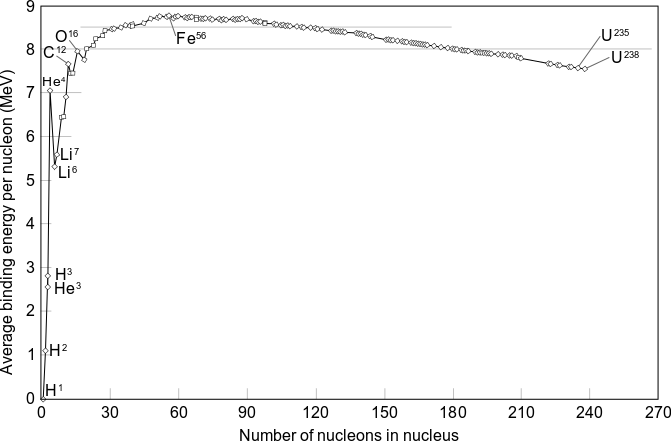
\includegraphics[width=0.75\linewidth]{Kap2/Figures/Binding_energy_curve_-_common_isotopes.png}
    \caption{This figure shows the binding energy per nucleon as a function of the number of nucleons. From \textbf{Ref.} \cite{BEPN_figure}}
    \label{fig:BE_energy_per_nucleon}
\end{figure}

Processes that result in nuclei with more binding energy per nucleon convert mass into energy \cite{Stacey_2010}. There are two possible processes in which this may happen: fission and fusion reactions. Fusion reactions happen when two light nuclei combine and form a heavier nucleus \cite{Lewis_2014}. On the contrary, fission occurs when a heavier nucleus splits to form lighter nuclei \cite{Stacey_2010}. Fission is the process on which nuclear reactors are based.

\subsection{Liquid-Drop Model}
The liquid-drop model, one of the first nuclear models, was proposed by Bohr in 1935. It is based on the short range of nuclear forces as well as the additivity of volumes and binding energies. The basic idea is that nucleons interact strongly with their neighbours, similar to how molecules interact in a drop of water \cite{Spiro}.

Based on this model, in 1935 Bethe and Weizs\"{a}cker made an excellent parametrization of the binding energies of nuclei in their ground state. This formula extends the idea of the liquid-drop model to incorporate two new ingredients, related to quantum properties of the nuclear mater. The first one is the asymmetric energy which tends to stabilize nuclei with equal number of protons and neutrons. The other is the pairing energy which favors paired fermions \cite{Spiro}. The formula is composed by five therms:

\begin{itemize}
    \item The first parameter in the formula is related to the volume ($a_{v} = 15.753 MeV$). This term reflects the nearest neighbor interactions and leads to a constant binding energy per nucleon.
    \item The term $a_{s}$ lowers the binding energy and is related to the surface of the nucleus. While internal nucleus feel isotropic interactions, nucleus on the surface feel forces coming only from the inside. Since superficial area of a sphere is $4\pi R^2$ and $R \sim A^{2/3}$, this therm is proportional to $A^{2/3}$.
    \item $a_{c}$ is related to the Coulomb repulsion of protons therefore lowers binding energy of the nucleus. Coulomb potential is proportional to $Q^2/R$ thus $a_{c} \sim Z^2/A^{1/3}$.
    \item While $a_{c}$ favors neutron excess over protons, the term $a_{a}$ favors symmetry between protons and neutrons related to the isospin.
    \item Finally, $\delta(A)$ is a quantum pairing term.
\end{itemize}

The Bethe-Weizs\"{a}cker's formula is:\cite{Spiro}

\begin{flalign}
    && B(A,Z) = a_{v}A - a_{s}A^{2/3} - a_{c} \frac{Z^2}{A^{1/3}} - a_{a} \frac{(N-Z)^2}{A} + \delta(A) &&
    \label{eq:binding_energy_ldm}
\end{flalign}

Since this is a empirical formula each parameter $a_{i}$ has to be fitted to the data. This fitting process results in the following values:

\begin{itemize}
    \item $a_{v} = 15.753 MeV$
    \item $a_{s} = 17.804 MeV$
    \item $a_{c} = 0.7103 MeV$
    \item $a_{a} = 23.69 MeV$
    \item $\delta(A) =
        \begin{cases} 
        33.6A^{-3/4} & \text{if } N \text{ and } Z \text{ are even} \\
        -33.6A^{-3/4} & \text{if } N \text{ and } Z \text{ are odd} \\
        0 & \text{if } A = N + Z \text{ is odd}
        \end{cases}$
\end{itemize}

\subsection{Instability of Isotopes}

Induced fission occurs when a probe transfers energy into a nucleus, leaving it in an excited state, which may then split into two fragments of similar size. There are various kinds of probe, but for induced fission reactions, neutrons are the most effective because they do not have an electric charge. Therefore, they do not experience Coulomb repulsion, allowing them to penetrate deeper into the nucleus, bringing energy and causing a rearrangement in the shell structure of the nucleus.\cite{Notas_sanabricas}

For instance suppose and spherical nucleus with:

\begin{flalign*}
    && V = \frac{4}{3} \pi R^3 &&\\
    && S = 4\pi R^2 &&
\end{flalign*}

We will explore the effects of a small deformation like an prolate spheroid. Since nuclear mater is incompressible, the volume will not change, at least to first order. Consider a small deformation, $\epsilon << 1$:

\begin{flalign*}
    && a = R(1+\epsilon) ;b = R(1+\epsilon)^{-1/2} &&\\
    && V = \frac{4}{3} \pi ab^2 = \frac{4}{3} \pi R^3 && 
\end{flalign*}

With these definitions, the volume remains constant, but the surface area increases. Using a Taylor series expansion for small $\epsilon$, we have:

\begin{flalign*}
    && \frac{a}{b} = 1 + \frac{3}{2} \epsilon + \frac{3}{8} \epsilon^2 + \dotsb &&
\end{flalign*}

Also,

\begin{flalign*}
    && \left(\frac{b}{a}\right)^2 = 1 - 3 \epsilon + 6 \epsilon^2 - 10 \epsilon^3 + \dotsb &&
\end{flalign*}

Given $\frac{\arcsin \epsilon}{\epsilon} = 1 + \frac{1}{2} \epsilon - \frac{13}{40} \epsilon^2 + \dotsb$, we get:

\begin{flalign*}
    && \left(\frac{b}{a}\right)^2 \left(\frac{\arcsin \epsilon}{\epsilon}\right) = 2\left(1 + \epsilon + \frac{2}{3} \epsilon^2 + \dotsb\right) &&
\end{flalign*}

Substituting into the surface area $S$:

\begin{flalign}
    && S = 4\pi R^2 \left(1 + \frac{2}{5} \epsilon + \dotsb\right) &&
    \label{eq:S_binding_deformed}
\end{flalign}

Finally, considering the average distance between nucleons inside the deformed nucleus:

\begin{flalign}
    && \Bar{R} &= R \left(1 + \frac{1}{5} \epsilon^2 + \dotsb\right) \nonumber && \\
    && \Bar{R}^{-1} &= R^{-1} \left(1 - \frac{1}{5} \epsilon^2 + \dotsb\right) &&
    \label{eq:R_binding_deformed}
\end{flalign}

Knowing how $\Bar{R}$ and S change in the nucleus with the small deformation \textbf{Eq.}(\ref{eq:R_binding_deformed})  and \textbf{Eq.}(\ref{eq:S_binding_deformed}) respectively, we can evaluate the binding energy \textbf{Eq.}(\ref{eq:binding_energy_ldm}) and see how it changes. The Coulomb and the surface terms are the ones that change. The following analysis will detail these changes:

\begin{flalign*}
    && \Delta E = B(\epsilon) - B(0) &&\\
    && \Delta E = \left(-\frac{2}{5}a_{s}A^{2/3} +\frac{1}{5} a_{c} z (z-1) A^{-1/3} \right) \epsilon^2 &&
\end{flalign*}

If $\Delta E > 0$, then $B(\epsilon) > Bb(\epsilon = 0)$. This means that the deformed nucleus is lighter that the spherical one, resulting in an tendency towards stretching in the nucleus, which leads to fission \cite{Krane}. We will focus on the conditions that lead to $\Delta E > 0$:

\begin{flalign*}
    && -\frac{2}{5}a_{s}A^{2/3} +\frac{1}{5} a_{c} z (z-1) A^{-1/3} > 0 &&\\
    && \frac{1}{5} a_{c} z (z-1) A^{-1/3} > \frac{2}{5}a_{s}A^{2/3} &&\\
    && \left( z \gtrsim 90 \right) \rightarrow z(z-1) \approx z^2 &&\\
    && a_{c} Z^2 > 2 a_{s} A && \\
    && Z^2/A > \frac{2 a_{s}}{a_{c}} &&
\end{flalign*}

The right side of the expression can be approximated $\frac{2 a_{s}}{a_{c}} \approx 47$ which leave us we the condition \cite{Krane}:

\begin{flalign}
    && \frac{Z^2}{A} > 47. && 
    \label{eq:inestability}
\end{flalign}

A nucleus with this property is completely unstable to fission. When discussing about nuclear reactors, we want isotopes that are prone to fission, but this probability should not be too high because spontaneous fission would dominate the reaction, reducing the efficiency of the reactor \cite{Notas_sanabricas}. Nuclei with $Z>90$ and $A>230$ undergo fission relatively easily, either through induced or spontaneous processes.\cite{Lewis_2014}

\subsection{Valley of Instability}

The presence of Coulomb and asymmetric terms in the binding energy \textbf{Eq.}(\ref{eq:binding_energy_ldm}) implies the existence of a maximum in the binding energy for a given \( A \), as a function of \( Z \) \cite{Spiro}. To find this relation, we set \(\partial B/\partial Z = 0\), as shown in the following expression:

\begin{flalign*}
    && \frac{\partial B}{\partial Z}\bigg|_{A=\text{const}} = -2a_{c} \frac{Z_{\text{min}}}{A^{1/3}} + 2 a_{a} \frac{(N-Z_{\text{min}})}{A} &&
\end{flalign*}
Setting this expression to zero and replacing \(N = A-Z\), we get:
\begin{flalign*}
    && 0 = -2a_{c} \frac{Z_{\text{min}}}{A^{1/3}} + 2 a_{a} \frac{(A-2Z_{\text{min}})}{A} && \\
    && 0 = - a_{c} \frac{Z_{\text{min}}}{A^{1/3}} + a_{a} - 2\frac{Z_{\text{min}}}{A} && \\
    && Z_{\text{min}} = \frac{A}{2+a_{c}A^{2/3}/(2a_{a})} &&
\end{flalign*}

This expression can be approximated by \(N = Z = A/2\) and \(a_{c}/a_{a} \approx 0.0075\) \cite{Spiro}. This leaves us with the expression:

\begin{flalign}
    && Z_{\text{min}} \approx \frac{A}{2} \, \frac{1}{1+0.0075 \, A^{2/3}} &&
    \label{eq:stability_valley}
\end{flalign}

The \textbf{Eq.}(\ref{eq:stability_valley}) tells us which is the most stable isotope for a given \( A \). This information will be helpful later in the document when we discuss the requirement of stable isotopes for the reactor fuel.



\section{Nuclear Fission}
A first approximation to study the probability of a nuclear fission, one can suppose that the fission fragments live within the nucleus and fission takes place when one of them surpasses the Coulomb barrier \cite{Notas_sanabricas}.

For instance, consider the fission reaction of a nucleus, specifically $\prescript{235}{}{U}$ undergoing an induced fission reaction. We will delve into this type of fission later in the document. This reaction results in many products such as neutrons, fission fragments and radiation, as shown in \textbf{Fig} (\ref{fig:fission_react}). Each of these products plays its role in a nuclear reactor.

\begin{figure}[h]
    \centering
    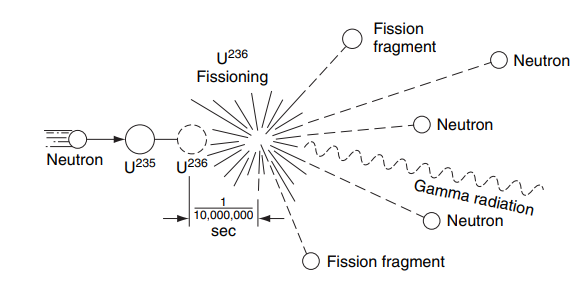
\includegraphics[width=0.75\linewidth]{Kap2/Figures/fission_reaction_stacey.png}
    \caption{Detailed Schematic of a Nuclear Fission Reaction. From \textbf{Ref.} \cite{Stacey_2010}.}
    \label{fig:fission_react}
\end{figure}

Subsequently, suppose that the nucleus splits in two similar fragments, $\prescript{119}{46}{Pd}$. To compute the energy liberated in the reaction we just need to compute the difference in binding energy between $\prescript{238}{}{U}$ and $2\times\prescript{119}{}{Pd}$, which is equal to 214 MeV.

To continue, we compute the Coulomb barrier, knowing that $R = R_{1} + R_{2}$,  $R_{2} = R_{1}$ and $R_1 = R_{0} (119)^{1/3} = 6\, \text{fm}$:

\begin{flalign*}
    && V = \frac{1}{4\pi \epsilon_{0}} \frac{Z_{1}Z_{2}e^2}{R} &&\\
    && R = 12\, \text{fm} &&\\
    && Z_1 = Z_2 = 46 &&\\
    && V = 253\, \text{MeV} &&
\end{flalign*}    


The excitation energy of the fragments inside $\prescript{238}{}{U}$ is 214 MeV and the height of the Coulomb barrier is 253 MeV. This values are not that different, which  makes the probability non-zero for one of the fragments escaping the nucleus because of quantum tunneling. This calculation is a mere sketch  of what a real calculation needs to consider. For example, if we choose the two fragments to be $\prescript{79}{30}{Zn}$ and $\prescript{159}{62}{Sm}$ the Coulomb barrier will be reduced to 221. In more sophisticated version of these calculations, two new parameters will be added:

\begin{itemize}
    \item Fission barrier 
    \item activation energy
\end{itemize}

These more sophisticated calculation are based on the liquid-drop model and give us an idea of the activation energy, the energy required for a nucleus to surpass the fission barrier and fission \cite{Krane}.

When a neutron is absorbed into a heavy nucleus resulting in a compound nucleus, the binding energy per nucleon decreases. For some nuclei, such as $\prescript{233}{92}{U}$, $\prescript{235}{92}{U}$, $\prescript{239}{92}{Pu}$, this decrease is so significant that the compound nucleus will undergo fission with high probability, even if the neutron has very low energy \cite{Stacey_2010}. A compound nucleus is an excited nucleus which decays via multiple paths, depending on the isotope.

\subsection{Fission Products}
Fission is an asymmetric process, this means the two resulting fragments have different masses. However, the probability that the two fragments have the same mass is close to zero, which is not well understand \cite{Notas_sanabricas}. 

\begin{figure}[h]
    \centering
    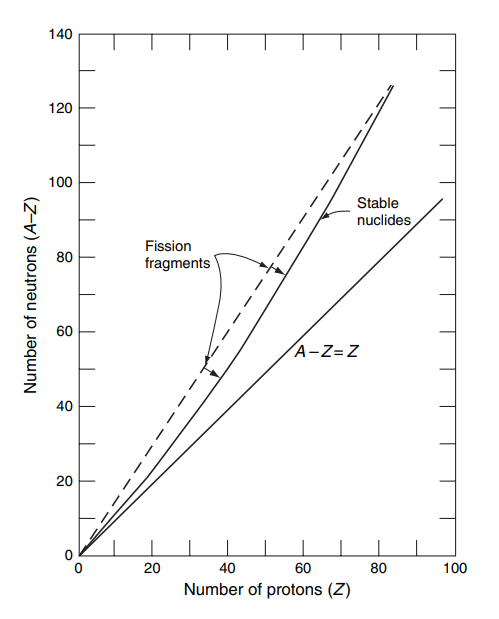
\includegraphics[width=0.5\linewidth]{Kap2/Figures/stability_curve.png}
    \caption{Graph illustrating the relationship between the number of neutrons and the number of protons in nuclei. From \textbf{Ref.} \cite{Lewis_2014}}
    \label{fig:Stability_curve}
\end{figure}

Fission fragments are unstable because they neutron excess \cite{Lewis_2014}. When a nucleus undergoes fission, it not only produces fragments but also emits neutrons, known as prompt neutrons. This emission changes the proton-to-neutron ratio of the fragments. Nonetheless, these fragments still lie about the stability curve in \textbf{Fig} (\ref{fig:Stability_curve}). Some of these nuclei, less than $1\%$, decay by delayed-neutron emission, most of the fragments decay via beta emission or gamma rays. For example:

\begin{flalign*}
    && n + \prescript{235}{92}{U} &\rightarrow \prescript{140}{54}{Xe} + \prescript{94}{38}{Sr} + 2n + 200MeV &&
\end{flalign*}

$\prescript{140}{54}{Xe}$ follows the chain of reactions:

\begin{flalign*}
    && \prescript{140}{54}{Xe} \xrightarrow{\beta} \prescript{140}{55}{Cs} \xrightarrow{\beta} \prescript{140}{56}{Ba} \xrightarrow{\beta} \prescript{140}{57}{La} \xrightarrow{\beta} \prescript{140}{58}{Ce} &&
\end{flalign*}

This process shows only one of the 40 possible pairs that results from fission \cite{Lewis_2014}. These fragments are highly radioactive and, in some cases, they can produced delayed neutron. Prompt and delayed neutrons play and fundamental role in the dynamics of a nuclear reactor.

\subsection{Fission Cross Sections}
Next we are going to focus on $\sigma$ known as the nuclear reaction cross-section, which is a value that quantifies the probability of a nuclear reaction occurring \cite{Stacey_2010}. This parameter is expressed in terms of the number of neutrons traveling with speed $v$ a distance $dx$ in a material with N nuclei per unit volume

\begin{flalign}
    && \sigma := \frac{\text{reaction rate}}{nvNdx} &&
\end{flalign}

$\sigma$ has units of area, consistent with the idea that $\sigma$ is an effective area of interaction. That is why is called `cross-section'. Typically, this parameter is measured in Barns. $1\text{barn} = 10^{-24} cm$ \cite{Stacey_2010}.

 The fission cross section ($\sigma_{f}$), represents the probability that the interaction of a neutron and a nucleus will result in fission \cite{Stacey_2010}. The probability peaks when the energy delivered to the nucleus, matches the energy difference between an excited state and the ground state of the compound nucleus. This phenomenon is known as resonances \cite{Stacey_2010}. 

$\prescript{238}{}{U}$ fissions only by \textit{fast neutrons} which are neutrons of high energy (energies around MeV). However, this cross section is small compared to others \cite{Notas_sanabricas}. On the other hand, $\prescript{235}{}{U}$ and $\prescript{239}{}{Pu}$ undergo fission with neutrons across all energy spectra present in a nuclear reactor \cite{Notas_sanabricas}, as shown in \textbf{Fig} (\ref{fig:Cross_section_fission}), including its resonances, which corresponds to the peaks in the graph.

\begin{figure}
    \centering
    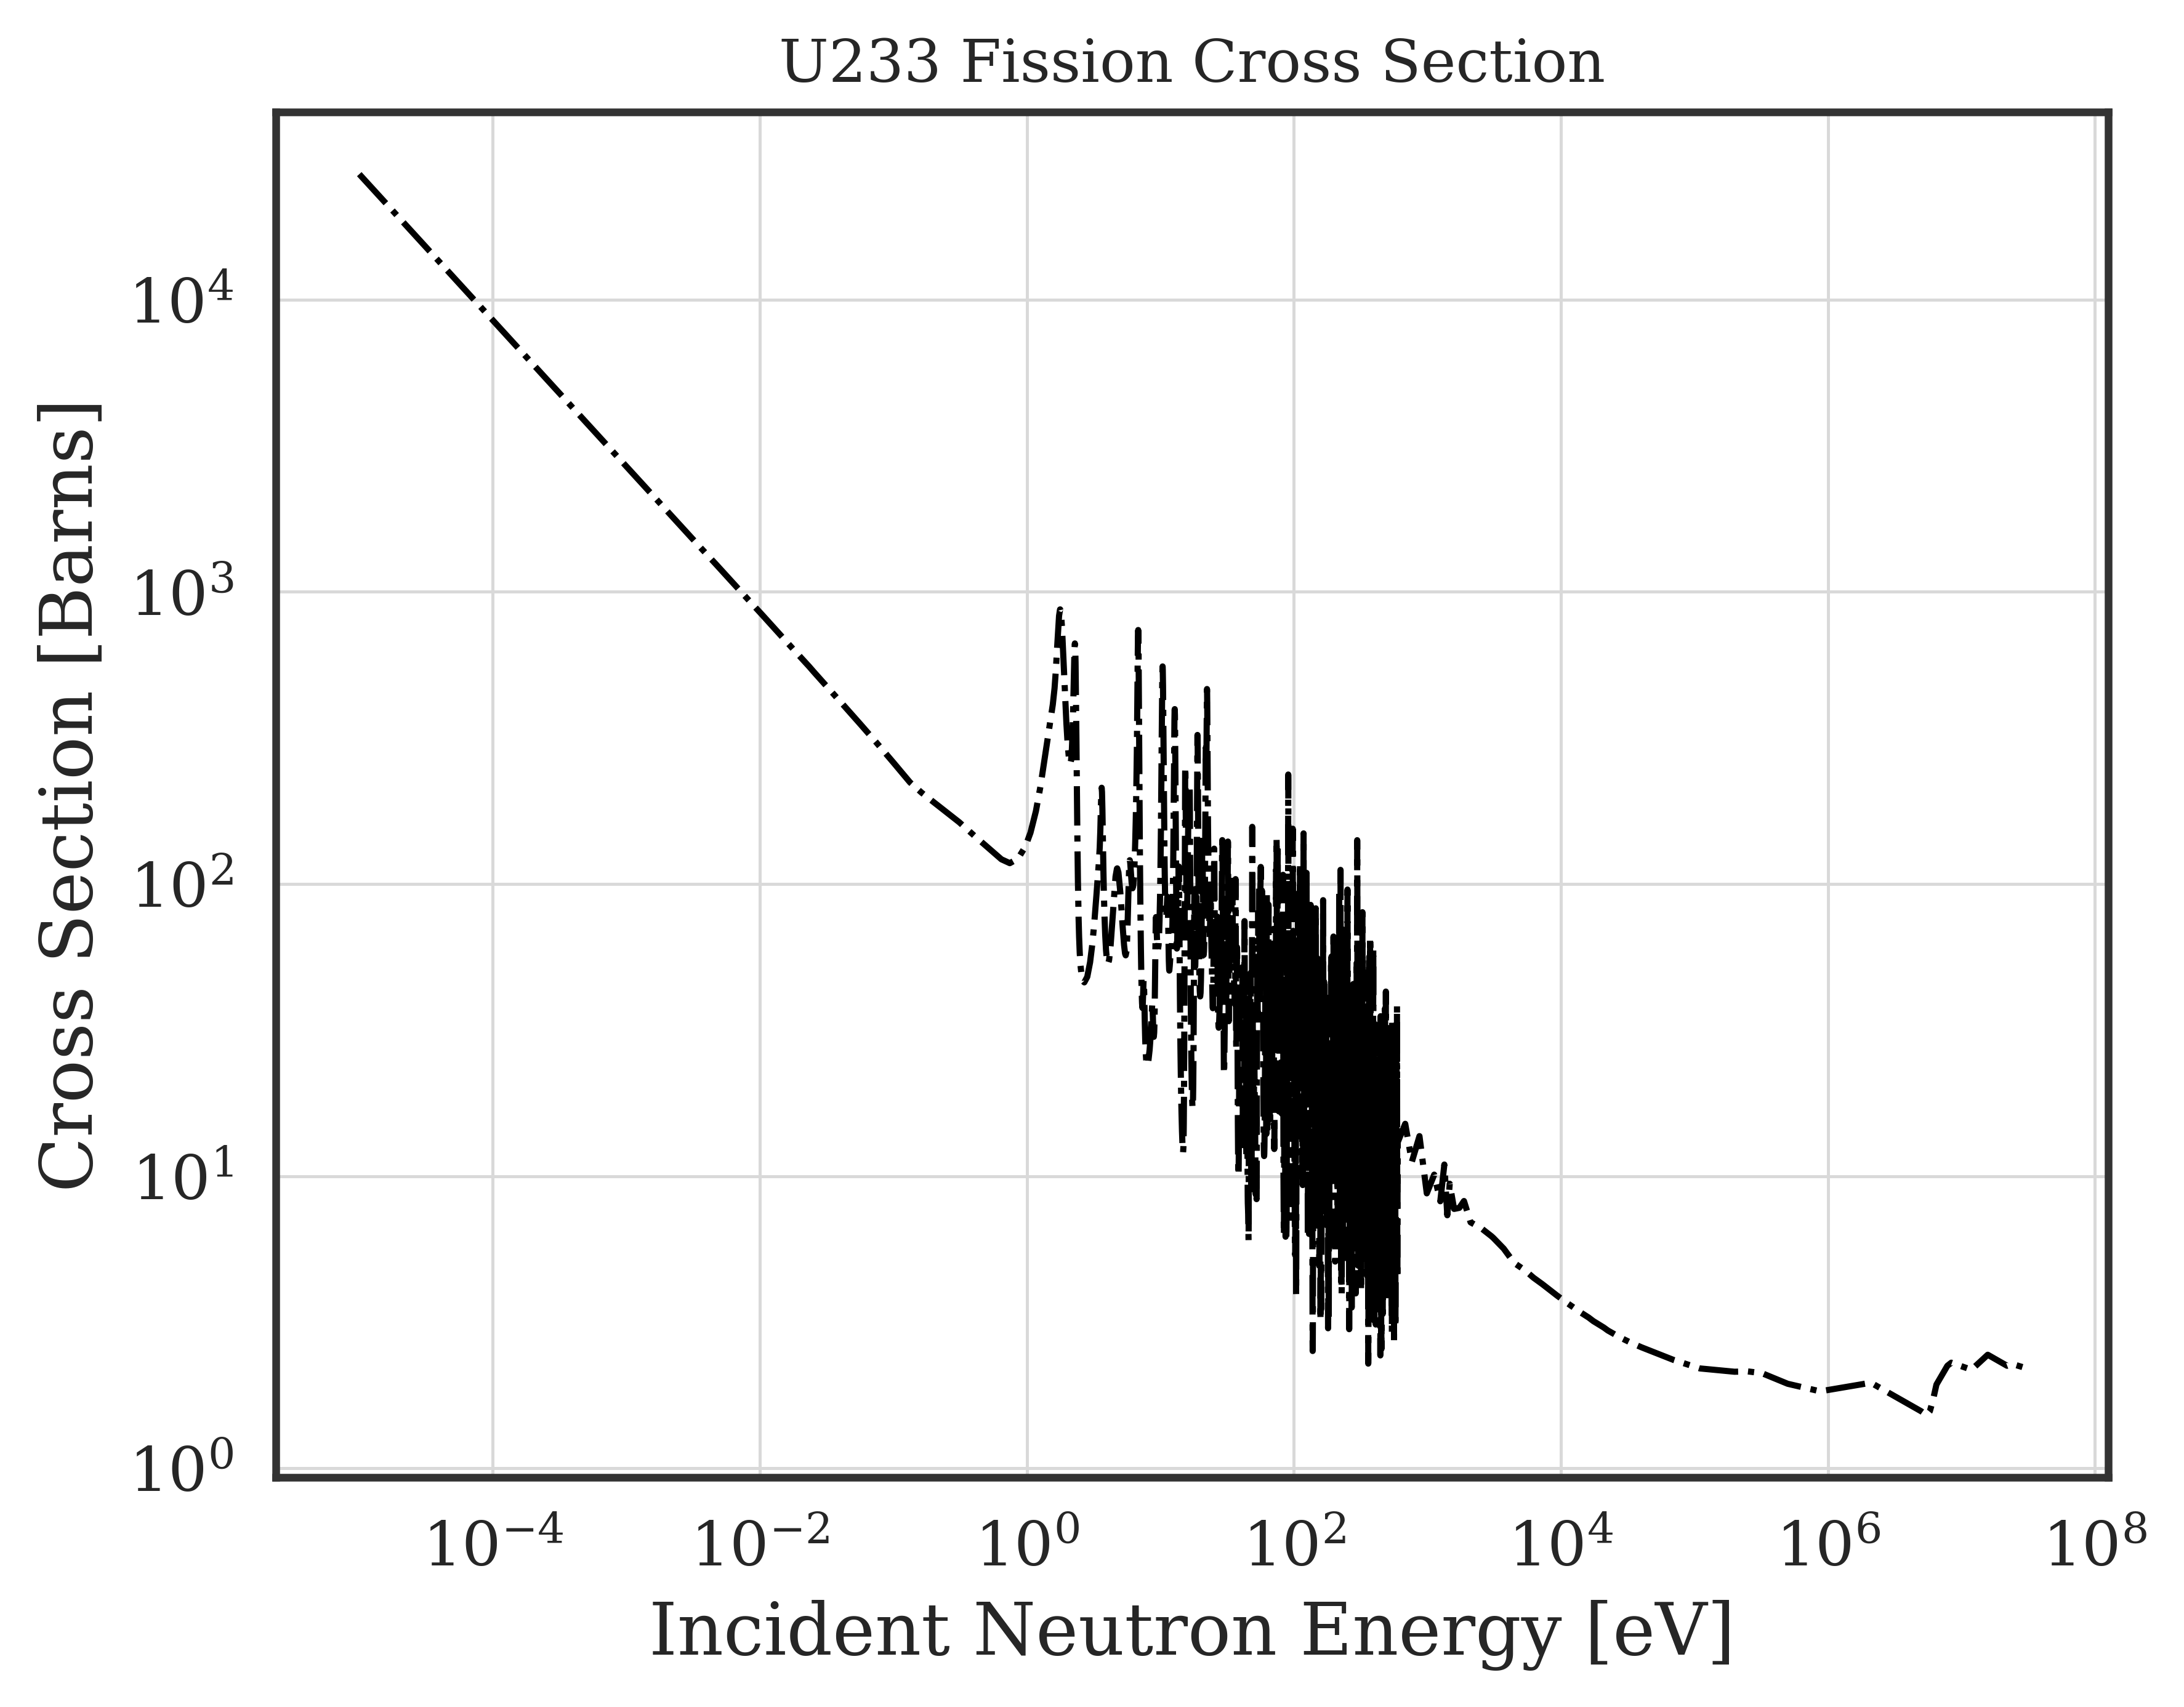
\includegraphics[width=0.75\linewidth]{Kap2/Figures/U233_Cross_Section.png}
    \caption{Fission cross section of $\prescript{233}{}{U}$. Data retrieved from \textbf{Ref.} \cite{NNDC}}
    \label{fig:Cross_section_fission}
\end{figure}

\section{Abundances of Isotopes}
\label{sec:possible_fuels}

We already explored the instability of isotopes. Relation \textbf{Eq.}(\ref{eq:inestability}) give us an idea of how prone is a nucleus to fission. For instance, if we compute this parameter for the following nuclei, we get:

\begin{align*}
    \prescript{208}{82}{Pb} \rightarrow 32.33\\
    \prescript{232}{90}{Th} \rightarrow 34.91\\
    \prescript{238}{92}{U} \rightarrow  35.56\\
    \prescript{235}{92}{U} \rightarrow 36.02\\
    \prescript{233}{92}{U} \rightarrow 36.33\\
    \prescript{239}{94}{Pu} \rightarrow 36.97\\
    \prescript{252}{94}{Cf} \rightarrow 38.11
\end{align*}

All isotopes can undergo fission if they are hit with enough energy. In nuclear physics, probes usually have kinetic energies around MeV. Lead (Pb) is a very stable isotope. Isotopes, including Thorium-232 ($\prescript{232}{}{Th}$) and Uranium-238 ($\prescript{238}{}{U}$), have a non-zero probability of fission, yet their cross-sections are small. In contrast, isotopes, such as $\prescript{235}{}{U}$, $\prescript{233}{}{U}$ and $\prescript{239}{}{Pu}$, are more prone to fission. Nuclei over Plutonium (Pu) can undergo spontaneous fission. This condition worsens for isotopes with $Z^2/A \geq 39$ which have infinitesimally small mean life \cite{Notas_sanabricas}. Bringing this in mind, we can estimate some ranges for the stability of isotopes:
\begin{center}
\begin{align*}
    Z^2/A < 35 &\rightarrow \text{Too stable}\\
    Z^2/A \sim 35 &\rightarrow \text{Fissile but not that much}\\
    Z^2/A \sim 36 &\rightarrow \text{Prone to fission}\\
    Z^2/A \sim 38 &\rightarrow \text{Spontaneous fission}\\
    Z^2/A  \gtrsim 39 &\rightarrow \text{Too unstable} \\
    Z^2/A > 47 &\rightarrow \text{Not possible}
\end{align*}
\end{center}

Besides, we have to look for isotopes that are close to the bottom of the valley of stability \textbf{Eq.} (\ref{eq:stability_valley}). Those far away from the valley will decay via $\beta^{+/-}$, $\alpha$, neutron or proton evaporation \cite{Notas_sanabricas}. This leaves us with three possible isotopes:

\begin{center}
\begin{align*}
    \prescript{233}{}{U} &\rightarrow \tau = 160000 \, \text{years}\\
    \prescript{235}{}{U} &\rightarrow \tau = 700  \, \text{million years}\\
    \prescript{239}{}{Pu} &\rightarrow \tau = 24000  \, \text{years}
\end{align*}
\end{center}

For an approximation of how much of each material is available on Earth, we are going to compare their mean life with the lifespan of Earth which is around $4.54$ billion years. $\prescript{239}{}{Pu}, \tau = 24000 \, \text{years}$ This means it has passed $187000$ mean lifespans since the creation of Earth, which indicates there is no plutonium left on earth. Something similar happens for $\prescript{233}{}{U}$. Quite the contrary is the case of $\prescript{235}{}{U}$ which has a mean life comparable to earth's age, which means there is $\prescript{235}{}{U}$ on the planet but not that much.

The uranium available on Earth is known as `natural uranium' ($\prescript{Nat}{}{U}$). Its composition is : 

\begin{equation*}
    \begin{cases}
        \prescript{238}{}{U} &\rightarrow 99.274\%\\
        \prescript{235}{}{U} &\rightarrow 0.720\%\\
        \prescript{234}{}{U} &\rightarrow 0.005\%
    \end{cases}
\end{equation*}

These isotopes are the ones that could be used as initial nuclear fuel for a nuclear reactor \cite{Notas_sanabricas}.

\subsection{Notation}

Latter on this document an special notation will be used to indicate the isotopes discussed here. The reader may notice the following pattern:

\begin{align*}
    Th \rightarrow Z=90\\
    Pu \rightarrow Z=94\\
    Z \in [90,94]
\end{align*}

As well as :

\begin{align*}
    \prescript{232}{}{Th} \rightarrow A = 232\\
    \prescript{239}{}{Pu} \rightarrow A = 239\\
    A \in [232, 239]
\end{align*}

So we can think that we have the `general case':

\begin{equation*}
    \prescript{23b}{9a}{X} \rightarrow \begin{cases}
        a = 0,1,2,3,4\\
        b = 2,3,4,5,6,7,8,9
    \end{cases}
\end{equation*}

So we can use this two numbers to refer to a certain isotope. For example:

\begin{align*}
    \prescript{232}{90}{Th} &\rightarrow 02\\
    \prescript{235}{92}{U} &\rightarrow 25\\
    \prescript{238}{92}{U} &\rightarrow 28
\end{align*}

\subsection{Fissionable and Fertile Material}

Having introduced the fuel of a nuclear reactor, now we have to distinguish between two sub classes of fissionable material. Firstly, we have fissile nuclei which are the ones that undergo fission when they are irradiated by neutrons of some energy. For example $\prescript{235}{}{U}$ is fissile. Secondly, we have fertile material which can undergo fission only by high energy neutrons. However, fertile materials can become fissile if they captures neutrons, trans-mutating via $\beta$ decays or capturing neutrons again. This is the case of Thorium-232 ($\prescript{232}{}{Th}$) and Uranium-238 ($\prescript{238}{}{U}$).

\begin{flalign*}
    && n + \prescript{238}{92}{U} \rightarrow \prescript{239}{92}{U}^{*} \xrightarrow{\beta^{-}} \prescript{239}{93}{Np} \xrightarrow{\beta^{-}} \prescript{239}{94}{Pu} &&
\end{flalign*}

\begin{flalign*}
    && n + \prescript{232}{90}{Th} \rightarrow \prescript{233}{90}{Th}^{*} \xrightarrow{\beta^{-}} \prescript{233}{91}{Pa} \xrightarrow{\beta^{-}} \prescript{233}{92}{U} &&
\end{flalign*}

The crust of Earth has at least three times more Thorium-232 than Uranium \cite{IAEA2005}. Using this material to breed $\prescript{233}{}{U}$ is the idea behind a Thorium fuel cycle. However, a breeding chain reaction is more difficult to sustain than a fission chain reaction \cite{Notas_sanabricas}.

\section{Neutron Interactions}

In order to produce energy, a nuclear reactor must sustain an equilibrium between the neutrons generated within the core and the neutrons lost\cite{Lamarsh_Baratta_2009}.To achieve this, a nuclear reactor must sustain an induced fission chain reaction. In this process, neutrons, produced by fission, induced new fissions in other fissile nuclei \cite{Lamarsh_Baratta_2009}. These new fissions produce more neutrons, which induce further reactions, repeating the process. \textbf{Fig} (\ref{fig:chain_reaction}) illustrates this process.

In each fission of $\prescript{235}{}{U}$, an average of 2.4 neutrons are produced \cite{Lewis_2014}. We have already seen that around $200$ MeV of energy is liberated after the fission of $\prescript{235}{}{U}$. Nonetheless, this energy is released as kinetic energy of the fission fragments (FF) and is eventually dissipated as heat.

\begin{figure}[h]
    \centering
    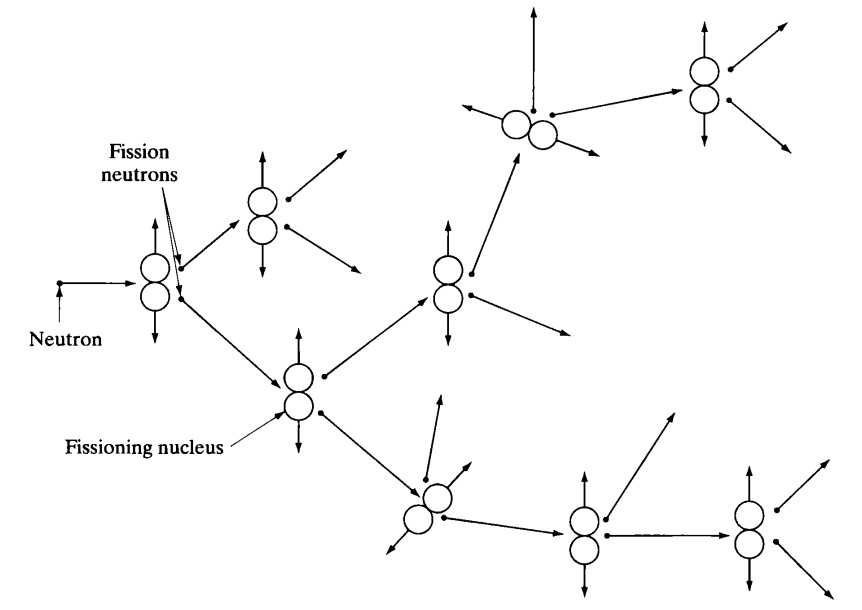
\includegraphics[width=0.75\linewidth]{Kap2/Figures/Chian_reaction.png}
    \caption{Fission reaction chain schematic. From \textbf{Ref.} \cite{Lewis_2014}}
    \label{fig:chain_reaction}
\end{figure}

\subsection{Neutron Multiplication}

The reaction represented in \textbf{Fig} (\ref{fig:chain_reaction}) can be described in terms of a parameter known as `multiplication factor', denoted as \(k\) \cite{Lewis_2014}. The factor is defined as the number of neutrons produced in one generation divided by the number of neutrons produced in the preceding generation.

\begin{flalign}
    && k := \frac{\text{Number of fission's neutrons produced in one generation}}{\text{Number of fission's neutrons produced in the preceding generation}} &&
    \label{eq:def_multiplicative_factor}
\end{flalign}


In addition, if we want to estimate the number of neutrons produced in one generation, we need to use \(l\), which is the lifespan of a neutron inside the reactor \cite{Lewis_2014}. This is the time between the production and the absorption of neutrons. Suppose that there are $n_0$ neutrons at $t=0$, then, we can use the following formula to compute the number of neutrons of the \(ith\) generation:

\begin{flalign}
    && n(t) = n_0 k^{t/l} &&
\end{flalign}

There are three possibilities for the values of \(k\):

\begin{center}
$
    k= \begin{cases}
        k > 1 : \text{``Supercritical''. Neutrons increases exponentially.}\\
        k = 1 : \text{``critical''. The number of neutrons remains constant.}\\
        k < 1 : \text{``Subcritical''. The number of neutrons decreases.}
    \end{cases}
$
\end{center}

\subsection{Heat Produced by the Fuel}

Around \(8\%\) of the 200 MeV of the energy produced by fission corresponds to the gamma rays associated with the beta decays of fission products \cite{Lewis_2014}. Therefore, after a shutdown, a reactor that has been operating a for a time will keep radiating a significant amount of heat \cite{Lewis_2014}. The heat produced after shutdown due to beta and gamma decays could be computed using the Wigner-Way formula.

\begin{flalign}
    && P_{d}(t) = 0.0622 P_{0}[t^{-0.2}+(t_{0}+t)^{-0.2}] &&
    \label{eq:heat_decays}
\end{flalign}

Where \(P_{d}(t)\) is the power generated at time \(t\), \(P_{0}\) is the power of the reactor before the shutdown and \(t_{0}\) is the time of power operation before the shutdown. Due to the decay heat produced after the shutdown, the reactor must be refrigerated to prevent overheating for a considerable period of time \cite{Lewis_2014}.

\section{Microscopic and Macroscopic Cross Sections}

After the previous discussion on nuclear fuel, we want to determine how neutrons interact with the material inside the reactor. To achieve this, let us consider a beam of neutrons traveling in the \(+x\) direction. The intensity of the beam is given by $I = n'''v$, where $n'''$ \footnote{In this notation, quantities marked with triple primes (\('''\)) represent volumetric densities, double primes (\(''\)) indicate surface densities, and single primes (\('\)) denote linear densities.} is the volumetric neutron's density and \(v\) is the velocity at which all of the neutrons are traveling \cite{Lewis_2014}.

We assume that a neutron that collides with a nucleus is either absorbed or scattered into a different direction, reducing the number of neutrons traveling in the same direction \cite{Lewis_2014}. This causes a decline in the intensity of the beam.

Let \(I(x)\) be the intensity of the beam after penetrating a distant x in the material. Then, if the beam travels an additional infinitesimal distance \(dx\), some neutrons will be removed. This removal is proportional to the number of nucleus in this region denoted as \(N\) and the cross-section, $\sigma$ \cite{Lewis_2014}. Therefore, we have:

\begin{flalign*}
    && I(x + dx) = (1 - N\sigma dx)I(x) &&
\end{flalign*}
If $I(0) = I_{0}$ and applying the derivative:

\begin{flalign*}
    && \frac{d}{dx} I(x) = -N\sigma I(x) &&
\end{flalign*}

Solving the differential equation an integrating from 0 to x:

\begin{flalign}
    && I(x) = I_{0}e^{-N\sigma x} &&
    \label{eq:mics_collided_flux}
\end{flalign}

\subsection{Macroscopic Cross Section}

After this result, we want to introduce the macroscopic cross section, defined as:

\begin{flalign}
    && \Sigma := N\sigma &&
    \label{eq:def_macs}
\end{flalign}

Where $\sigma$ refers to the microscopic cross section, measured in $cm^2/nucleus$, and N is still the volumetric nuclei density, measured in $nuclei/cm^3$. Then, the macroscopic cross section must have units of $cm^-1$.

Replacing $N\sigma$ in \textbf{Eq.}(\ref{eq:mics_collided_flux}) with $\Sigma$, we obtain a macroscopic version of the flux. We can interpret this collided flux as a probabilistic distribution indicating the likelihood of a neutron reaching a depth \(x\) into a material without colliding \cite{Lewis_2014}.

\begin{flalign*}
   && I(x) = I_{0}e^{-\Sigma x} &&
\end{flalign*}

Dividing \(I(x)\) by \(I_{0}\), we obtain the fraction of neutrons that have reached a distance \(x\) without colliding. Interpreting \(\frac{dI}{dx} = - \Sigma I(x)\) as the probability of a neutron having its first collision in the next \(dx\), we have:


\begin{flalign*}
   && p(x)dx = (\Sigma dx) (\frac{I(x)}{I_{0}}) = \Sigma e^{-\Sigma x} dx &&
\end{flalign*}

We can compute the mean free path \(\lambda\), the mean distance traveled by a neutron between collisions, as \cite{Lewis_2014}:

\begin{flalign*}
    && \lambda = \int_{0}^{\infty}xp(x)dx = \int_{0}^{\infty}x\Sigma e^{-\Sigma x}dx = \frac{1}{\Sigma} &&
\end{flalign*}

\section{Nuclei Density (N)}

The Avogadro's number is the total of molecules in a mole of a substance, $N_0 = 0.6023 \cdot 10^24$ \cite{Lewis_2014}. In order to compute the  density of the molecule of a substance, we have to divide $N_0$ by the molecular wight \(A\) and, finally, multiply it by the density of the substance \(\rho\) \cite{Lewis_2014}:

\begin{equation*}
    N = \rho N_{0}/A
\end{equation*}

Replacing this in \textbf{Eq.}(\ref{eq:def_macs}) we have:

\begin{equation*}
    \Sigma = \frac{\rho N_{0}}{A}\sigma
\end{equation*}

Now if we apply this formula to an chemical element we have to consider that this element, in reality, exist in nature as a mixture of isotopes. To adjust the formula to this case we denote $N^{i}/N$ as the atomic fraction of the isotope with $A_i$ atomic weight, Thus we define the atomic weight of the mixture as \cite{Lewis_2014}:

\begin{equation*}
    A = \sum_{i} (N^{i}/N) A_{i} ,
\end{equation*}

where $N = \sum_{i}N^{i}$. Applying this to get the macroscopic cross section we get:

\begin{equation}
    \Sigma = \frac{\rho N_{0}}{A} \sum_{i}\frac{N^{i}}{N} \sigma^{i}
    \label{eq:chemical_mcs}
\end{equation}

Where $\sigma^{i}$ is the microscopic cross section of the \(ith\) isotope.

In many cases material are combined using volume fractions. Once again, we want to make adjustment to our equation to consider this situation. Let $V_{i}/V$ the volume fraction where $V = \sum_{i}V_{i}$, the cross section of the mixture is \cite{Lewis_2014}:

\begin{equation}
    \Sigma = \sum_{i}(V_{i}/V)N_{i}\sigma^{i}
    \label{eq:mcs_chemical_vf}
\end{equation}.

To compute each of the nuclei number density we make use of the density of the \(ith\) nuclei $\rho_{i}$ and its atomic weight $A_{i}$

\begin{equation*}
    N_{i} = \rho_{i}N_{0}/A_{i}
\end{equation*}

The expression in \textbf{Eq.}(\ref{eq:mcs_chemical_vf}) can be re written in terms of the macroscopic cross section of its components.

\begin{equation*}
    \Sigma = \sum_{i}(V_{i}/V)\Sigma^{i}
\end{equation*}

Where $\Sigma^{i} = N_{i}\sigma^{i}$. This expression can also be written in terms of mass fractions. Applying the same idea as before we get:

\begin{equation*}
    \sigma = \sum_{i}(M_{i}/M) \frac{\rho N_{0}}{A_{i}} \sigma^{i}
\end{equation*}

Where $M_i/M = \rho_{i}V_{i}/(\rho_{i}V)$ is the mass fraction, $M = \sum_{i}M_{i}$ and $\rho = M/V$.

\subsection{Enriched Uranium}

We have already mentioned that in nature uranium is found as a mixture of two main isotopes: $99.3\%$ of $\prescript{238}{}{U}$ and $0.7\%$ of $\prescript{235}{}{U}$. However, in a nuclear reactor, enriched uranium is needed which is uranium where the mass fraction of $\prescript{235}{}{U}$ has been increased. We denote the enrichment as \cite{Lewis_2014}:

\begin{flalign}
    && \Tilde{e_a} = \frac{N^{25}}{(N^{25}+N^{28})} &&
    \label{eq:Atomic_enr}
\end{flalign}

This expression is known as the atomic enrichment, and from the definition, we can deduced that $1-\Tilde{e_{a}} = N^{28}/(N^{28}+N^{25})$ is the Uranium-238 fraction. We can compute the macroscopic cross section using the enrichment as follows \cite{Lewis_2014}:

\begin{flalign*}
   && \Sigma^{U} = \frac{\rho_{U}N_{0}}{\Tilde{e_{a}}235 + (1-\Tilde{e_{a}})238}[\Tilde{e_{a}}\sigma^{25}+(1-\Tilde{e_{a}})\sigma^{28}] &&   
\end{flalign*} 

Another definition way to defined the enrichment is using the masses:

\begin{flalign*}
    && \Tilde{e_{w}} = \frac{M^{25}}{(M^{28}+M^{25})} &&
\end{flalign*}

We can also get the mass fraction for $\prescript{238}{}{U}$ based on the enrichment by $1-\Tilde{e_{w}} = \frac{M^{28}}{(M^{25}+M^{28})}$. Using this definition to compute the macroscopic cross section:

\begin{flalign*}
    && \Sigma^{U} = \rho N_{0} \left[ \frac{1}{235}\Tilde{e_{w}}\sigma^{25} + \frac{1}{238}(1-\Tilde{e_{w}})\sigma^{28}\right] && 
\end{flalign*}

There exits a relation between $\Tilde{e_{a}}$ and $\Tilde{e_{w}}$. Using $N^{25} \sim M^{25}/235$ and $N^{28} \sim M^{28}/238$:

\begin{flalign*}
    && \Tilde{e_a} = \frac{\frac{M^{25}}{235}}{(\frac{M^{25}}{235}+\frac{M^{25}}{235})} &&\\
    && \Tilde{e_a} = \frac{\frac{1}{235}\frac{M^{25}}{M}}{(\frac{1}{235}\frac{M^{25}}{M}+\frac{1}{238}\frac{M^{28}}{M})} &&\\
    && \text{Using} \Tilde{e_{w} \sim \frac{M^{25}}{M}} \text{and} 1-\Tilde{e_{w} \sim \frac{M^{28}}{M}} &&\\
    && \Tilde{e_a} = \frac{\frac{238}{235}\Tilde{e_{w}}}{(\frac{238}{235})\Tilde{e_{w}}+(1-\Tilde{e_{w}})} &&
\end{flalign*}

which finally becomes:

\begin{flalign*}
    && \Tilde{e_a} = \frac{1.0128\Tilde{e_{w}}}{1+0.0128\Tilde{e_{w}}} &&
\end{flalign*}

Using the relation for a level $\Tilde{e_{w}} = 0.007$, the atomic enrichment would be $\Tilde{e_{a}} = 0.00709$, and the values gets closer the higher the enrichment. This means that the approximation $\Tilde{e_{w}} \approx \Tilde{e_{a}} \approx \Tilde{e}$ is accurate.

\section{Neutrons Cross Sections}

So far, we have only introduced the probability that a neutron interacts with a nucleus but we have not talked about the processes that could happened afterwards. The cross section introduced before is known as the total cross section an is denoted as $\sigma_{t}$. When a neutron hits a nucleus, it is either scatter or absorbed, this could be considered in our relations as \cite{Lewis_2014}:

\begin{flalign*}
    && \sigma_{f} = \sigma_{s} + \sigma_{a} &&
\end{flalign*}

In the expression $\sigma_{s}$ and $\sigma_{a}$ denotes the scattering and absorption cross sections. With this formulation of the total cross section we can easily compute the probability for given interaction to end in scattering or absorption using the fractions $\sigma_{s}/\sigma_{t}$ and $\sigma_{a}/\sigma_{t}$ respectively.  

However, the scattering cross section is divided further into elastic and inelastic scattering \cite{Lewis_2014}. In the inelastic scattering the neutron give energy to the nucleus leaving it in an excited state. Both kinds of scattering conserve momentum, but only elastic scattering conserve kinetic energy. This arises in the expression:

\begin{flalign*}
    && \sigma_{s} = \sigma_{n} + \sigma_{n'} &&
\end{flalign*}

Where $\sigma_{n'}$ denotes the cross section for the inelastic scattering.
Something similar happens with the absorption scattering. 

\begin{flalign*}
    &&b\sigma_{a} = \sigma_{\gamma} + \sigma_{f} &&
\end{flalign*}

We have two processes, the first one is the formation of a compound nucleus that does not re emit the neutron but eliminates its exited energy via gamma decays, denoted as $\sigma_{\gamma}$. This process is known as capture reaction and the remaining nucleus could be unstable and decay later on \cite{Lewis_2014}. The other process, more interesting for our application, is a fission process $\sigma_{f}$.

We express a particular macroscopic cross section using a sub index $x = s, a, \gamma, f$ which indicates the particular reaction that we are considering.

\begin{flalign*}
    && \Sigma_{x} = N\sigma_{x} &&
\end{flalign*}

\subsection{Neutron Energy Range}

We have talked about cross sections but we have not considered it energy dependence. In this case, their dependence refers to the energy of the neutron. First we have to establish an upper and a lower limit for the neutron's energy distribution.

\begin{itemize}
    \item Thermal neutrons: 0.001eV - 1.0 ev
    \item Intermediate neutrons: 1.0eV - 0.1MeV
    \item Fast neutrons: 0.1MeV - 10MeV
\end{itemize}

Neutron produced in a fission reaction follow a energy distribution. If $\chi$(E) is the energy distribution then a reasonable approximation of the distribution \cite{Lewis_2014}: 

\begin{flalign}
    && \chi(E) = 0.453 \exp{(-1.036E)}\sinh{(\sqrt{2.29}E)} &&
    \label{eq:dist_fission_neutrons}
\end{flalign}

Prompt neutrons suffer multiple collisions before being absorbed. The nuclei with which they collide follow a thermal distribution with \(E_{N} = \frac{3}{2}kT\), where \(T\) is the temperature of the reactor. Therefore, when neutrons collide, they lose energy, passing through an intermediate energy region. Eventually, those neutrons become thermal neutrons, which follow a Maxwell-Boltzmann distribution. These distributions are important because, later in the document, we will see the dependence of cross sections on energy, and this dependence can change the dynamics of the nuclear reactor.



